La librairie \textsc{Keras} est une interface Python/TensorFlow\cite{tf} permettant de manipuler des réseaux de neurones.
Ici, seul les fonctionnalités principales seront étudiées,
à savoir
création d'un réseau simple,
régression par \sgd\
et évaluation de performances.\\


Voici un exemple de réseau de neurone simple (\textsc{Figure}\ \ref{fig:net2})
qui va tenter d'apprendre l'application linéaire suivante : $f(X) = W\cdot X$.
Avec :
\begin{itemize}
    \item[\textbf{$X$ :}] le vecteur d'entrée tel que : $\dim(X) = 2$.
    \item[\textbf{$W$ :}] le vecteur de poids tel que : $w_1 = 0.2$ et $w_2 = 0.8$.
\end{itemize}
\begin{figure}[H]
    \center
    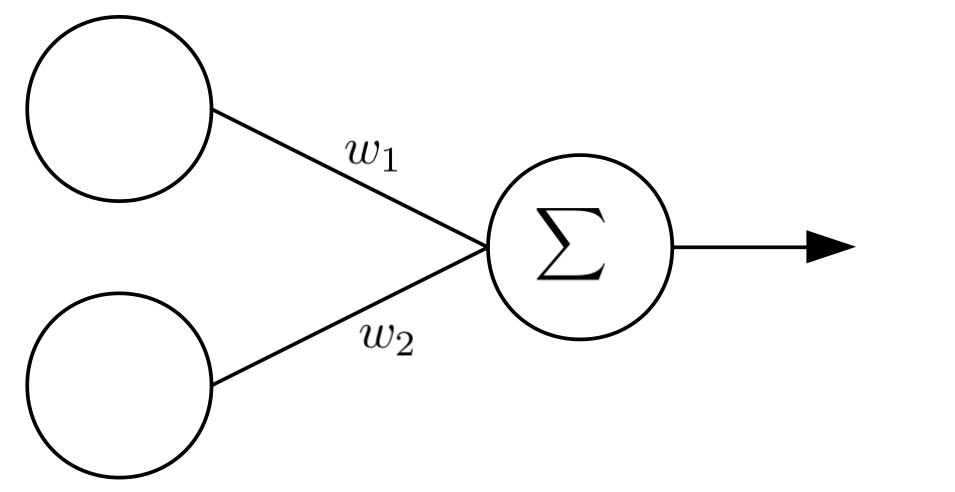
\includegraphics[height=\moyen]{pict/net2.png}
	\caption{Réseau simple}
    \vspace{-10pt}
    \begin{center}
        \footnotesize
        \textit{
        Avec $w_1 = 0.2$ et $w_2 = 0.8$.
        }
    \end{center}
	\label{fig:net2}
\end{figure}
\vspace{-12pt}


Pour créer ce réseau et lui faire apprendre la fonction précédemment citée,
le code suivant est nécessaire :
\newpage
\lstinputlisting[language=Python]{code/reseau1.py}


En exécutant ce code une fois, le résultat suivant est obtenu :
\begin{lstlisting}
w0 : 0.19988934695720673
w1 : 0.8001111745834351
\end{lstlisting}

Comme il peut être remarqué ci-dessus, les résultats obtenus sont proches de ceux attendus ($0.2$ et $0.8$).
La syntaxe de la librairie \textsc{Keras} est cependant assez lourde.
Une librairie a donc été codée pour simplifier son utilisation.
Elle pourra être appelée avec de nombreux paramètres qui seront abordés dans les parties suivantes.\\


Pour tester la robustesse de cet apprentissage, une fonction avec perturbations a été étudiée :
Une fonction simple a été générée comme précédemment, il y a été ajouté une perturbation aléatoire équiprobable.
L’erreur d’apprentissage en fonction de cette valeur a donc été étudiée.\\


\paragraph{Un problème se pose :}
Reprenons l'équation\ (\ref{eq:Choquet}) :
\begin{equation*}
    C_n (X) =
        \sum_{i=1}^{n}
                w_i \times x_i +
            \sum_{i=1}^{n}\sum_{j=i+1}^{n}
            \Big(
                w_{M\,ij} \times \max(x_i,x_j) + w_{m\,ij} \times \min(x_i,x_j)
            \Big)
\end{equation*}
Si on prend un vecteur de taille $n=2$, le résultat suivant est obtenu :
\begin{equation*}
    C_2 (X)
    =
        w_1.x_1 + w_2.x_2 + w_M.\max(x_1,x_2) + w_m.\min(x_1,x_2)
\end{equation*}
Étant donné que les données d'apprentissage sont des réels aléatoires indépendants entre $0$ et $1$ :
\begin{equation}
    \label{eq:proba}
    P(x_1 > x_2) = P(x_1 < x_2) = \frac{1}{2}
\end{equation}
Donc en combinant (\ref{eq:Choquet}) et (\ref{eq:proba}):
\begin{align*}
    \mathbb{E}(C_2 (X))
    & =
        w_1.x_1 + w_2.x_2 + \mathbb{E}(w_M.\max(x_1,x_2)) + \mathbb{E}(w_m.\min(x_1,x_2))
    &\\
    \mathbb{E}(C_2 (X))
    & =
        w_1.x_1 + w_2.x_2 + w_M.\frac{x_1 + x_2}{2} + w_m.\frac{x_1 + x_2}{2}
    &
\end{align*}
Et donc :
\begin{equation}
    \label{eq:obt}
    \mathbb{E}(C_2 (X)) =
        x_1 \times \Big(w_1 + \frac{w_m + w_M}{2}\Big) + x_2 \times \Big(w_2 + \frac{w_m + w_M}{2}\Big)
\end{equation}
Le réseau va donc tenter d'atteindre les valeurs solutions de l'équation
(\ref{eq:obt}) sans garantir l'exactitude des coefficients.

\exemle
{
Les deux quadruplés de valeurs suivantes vont genrer ce problème :
\begin{itemize}
    \item[Les bonne valeurs :] $(0.5, 0.25, 0.1, 0.15)$
    \item[D'autres valeurs :] $(0.28, 0.2, 0.33, 0.37)$
\end{itemize}
Si l'équation\ (\ref{eq:obt}) est appliquée sur cet exemple, le résultat suivant est obtenu :
\begin{table}[H]
    \centering
    \begin{tabular}{|l|l|l|}
        \hline
        Vecteur & $w_1 + \frac{w_m + w_M}{2}$ & $w_2 + \frac{w_m + w_M}{2}$ \\ \hline \hline
        $(0.5, 0.25, 0.1, 0.15)$  & $62.5$ & $37.5$ \\ \hline
        $(0.28, 0.2, 0.33, 0.37)$ &  $63$  &  $37$  \\ \hline
    \end{tabular}
    \label{tab:pb_tab}
    \caption{Valeurs retournées par les réseaux}
\end{table}
Les résultats du tableau précédent sont similaires :
en moyenne, le réseau ne les différenciera pas.
Il va donc apprendre a de mauvaises valeurs,
car en moyenne, le réseau à meilleurs résultats qu'avec des poids aléatoires.
C'est un minimum local de la fonction de perte.
}


Pour résoudre ce problème, il faut ne pas satisfaire l'équation (\ref{eq:proba})
pour supprimer l'équation (\ref{eq:obt}) et donc tirer un learning
set statistiquement différent du testing set.
De ce fait, si le réseau apprend ces mauvais poids, il sera instantanément pénalisé par le testing set.\\


Dans l'optique de minimiser le temps de calcul,
différentes fonctions de pertes ont été testées et comparées
(moindres carrés et erreur absolue).
Il a été étudié la variation de la precision du réseau en fonction des différentes fonctions de perte,
de si les données était triées et de la taille de la base de données.
